\documentclass[a4paper, 10pt]{article}
\usepackage[slovene]{babel}
\usepackage[utf8]{inputenc}
\usepackage{lmodern}
\usepackage[T1]{fontenc}
\usepackage{enumerate}
\usepackage{bbm}
\usepackage{graphicx}
\usepackage{subcaption}
\usepackage{float}
\renewcommand{\thefootnote}{\roman{footnote}}

\begin{document}
\begin{titlepage}
\title{Spektralno grupiranje}
\author{Špela Ognjanović in Žiga Trojer}
	\maketitle
\end{titlepage}


\section{Navodilo}
Implement spectral clustering algorithms that use several types of Laplace matrices. Consider unnormalized
spectral clustering, normalized spectral clustering according to Shi and Malik (2000), and normalized spectral clustering according to Ng, Jordan, and Weiss (2002). Generate various data sets or find some examples of real world data and use different types of similarity graphs such as complete graph, the
 $\epsilon$ -neighborhood graph and k-nearest neighbor graph. Compare the results.
Use different methods for determining the optimal number of clusters.

\section{Kratek opis}
Imamo bazo podatkov, naš cilj je te podatke razvrstiti v skupine oz. grupe s podobnimi lastnostmi. Podatke lahko prikažemo z grafi, grafe pa z matrikami. Eden takih primerov je \textbf{matrika sosednosti}, njena razsežnost je n $\times$ n. Element v \textsl{j}-tem stolpcu \textsl{i}-te vrstice pove število povezav, ki povezujejo točki \textsl{i} in \textsl{j}.

Predstavili bomo, kako lahko na različne načine pogrupiramo podatke, podane z množico točk \textsl{\ $x_1$, $x_2$, ... , $x_n$ } z utežmi $w_{i,j} \geq 0$, za $\forall i,j = 1, ... n$ ali razdaljami $d_{i,j} \geq 0$, za $\forall i,j = 1, ... n$. Če o podatkih nimamo veliko informacij, je najlažje, če jih predstavimo z grafom $G=(V, E)$. Vsako vozlišče $v_i$ predstavlja en podatek \textsl{$x_i$}. Potrebujem matriko, ki določa, kako blizu skupaj sta vozlišči $v_i$ in $v_j$. To matriko imenujemo podobna matrika in jo označimo s \textsl{S}. Dva vozlišča povežemo, če zadoščata danemu pogoju in to ponazorimo v podobnem grafu. Želimo, da imajo vozlišča v istih skupinah čim manjšo utežensot, kar pomeni da imajo podatki podobne lastnosti, sicer velja obratno. Spodaj so opisani trije primeri podobnih grafov, s katerimi bomo operirali.\\
\\
\textbf{Graf $\epsilon$ -ske okolice}\\
Pri $\epsilon$ -ski okolici grafa povežemo paroma vse točke, katerih razdalja je manjša od $\epsilon$. Največkrat je obravnavan kot graf brez uteži, saj nam utež predstavlja predpisana razdalja $\epsilon$.\\
\\
\textbf{Graf k najbližjih sosedov}\\
Cilj je, da povežemo vozlišče $v_i$ z njegovimi k najbližjimi sosedi. Dobimo, da je $v_i$ med k najbližjimi sosedi od $v_j$, obratno pa v splošnem ne velja.\\
\\
\textbf{Poln graf}\\
Je graf, kjer so vsa vozlišča med seboj povezana in utežena s $s_{i,j}$. Izbrana funkcija more modelirati lokalno sosednost, tako graf prikazuje lokalne sosedne razmere.\\
\\
Vrnimo se na podobno matriko \textsl{S}. Njene elemente izračunamo s pomočjo neke primerne funkcije. Primer take funkcije je Gauss-Karnelova funkcija, ki nam izračuna oddaljenost dveh vozlišč $v_i$ in $v_j$. Formula za izračun je:$$s(v_i, v_j) = exp(-\textbar\textbar v_i - v_j \textbar\textbar^2 / (2\delta^2)),$$pri čemer parameter $\delta$ opiše razdaljo med vozlišči, podobno kot $\epsilon$ pri grafu epsilonske okolice.  Vrednosti $s_{i,j}$, izračunane po tej meri, so na intervalu [0, 1]. Povejo nam, da manjša kot je vrednost, bolj sta točki oddaljeni. Če je vrednost 0, pomeni, da sta vozlišči daleč narazen. Matrika \textsl{S} je simertrična, saj za toliko kot je vozlišče $v_i$ oddaljena od vozlišča $v_j$, je tudi vozlišče $v_j$ oddaljena od vozlišča $v_i$. Očitno je, da so diagonalni elementi enaki 1.\\
\\
Naslednji korak je izračun \textbf{Laplaceove matrike}. Privzamemo, da imamo utežen, neusmerjen graf $G$. Uteži so prikazane v matriki \textsl{W}, $w_{i,j} \geq 0$, za $\forall i,j = 1, ... n$. Definirajmo stopnjo vozlišča $v_{i}\in V$: $$ d_i = \sum_{j=1}^n w_{i,j}.$$ Definiramo matriko stopenj $D$ kot diagonalno matriko s stopnjami vozlišč $d_{1},\ldots, d_{n}$ po diagonali.
\\
Glede na normalizirane in nenormalizirane ločimo dva primera Laplaceovih matrik:\\
\begin{enumerate}
\item\underline{Nenormalizirana Laplaceova matrika}, ki se izračuna po formuli $L=D-W$, kjer je \textsl{W} matrika uteži in \textsl{D} diagonalna matrika. Njene lastnosti so:
\begin{enumerate}[i)]
  \item Je simetrična, pozitivno semi-definitna.
  \item Njena najmanjša lastna vrednost je 0, njen pripadajoč lastni vektor je konstanten vektor $\mathbbm{1}$.
  \item Ima n nenegativnih, realni lastnih vrednosti $0 \leq \lambda_1 \leq ... \leq \lambda_n$.
  \item Za vsak $f \in\mathbbm{R}^n$ je $$f'Lf= \frac{1}{2} \sum_{i,j=1}^n w_{i,j}(f_i - f_j)^2.$$
\end{enumerate}

\item\underline{Normalizirana Laplaceova matrika} sta v bistvu dve matriki, ki sta med seboj povezani, prva je simetrična (zato oznaka $L_{sym}$) in se izračuna $L_{sym} = I - D^{-\frac{1}{2}}WD^{-\frac{1}{2}}$, druga pa je povezana z naključnim sprehodom (random walk), izračuna se po formuli $L_{rw} = I - D^{-1}W$.
Njune lastnosti so:
\begin{enumerate}[i)]
  \item Sta pozitivno semi-definitni in imata n nenegativnih, realnih lastnih vrednosti.
  \item 0 je lastna vrednost matrike $L_{rw}$, s pripradajočim konstantnim vektorjem $\mathbbm{1}$. 0 je tudi lastna vrednost matrike $L_{sym}$, s pripadajočim lastnim vektorjem $D^\frac{1}{2}\mathbbm{1}$.
  \item $\lambda$ je lastna vrednost matrike $L_{rw}$ z lastnim vektorjem $u$, natanko tedaj, če $u$ reši sistem $Lu = \lambda Du$.
  \item $\lambda$ je lastna vrednost matrike $L_{rw}$ z lastnim vektorjem $u$, natanko tedaj, če je $\lambda$ lastna vrednost matrike $L_{sym}$ z lastnim vektorjem $w = D^\frac{1}{2}u$.
  \item Za vsak  $f \in\mathbbm{R}^n$ je $$f'L_{sym}f= \frac{1}{2} \sum_{i,j=1}^n w_{i,j}(\frac{f_i}{\sqrt{d_i}} - \frac{f_j}{\sqrt{d_j}})^2.$$
\end{enumerate}
\end{enumerate}
Pri normalizirani in nenormalizirani Laplaceovi matriki je večkratnost $k$ lastne vrednosti 0 enaka številu povezanih komponent $A_{1},\ldots, A_{k}$.

\section{Načrt za reševanje}
Prednost algoritma spectral clustering je, da sestoji na preprosti linearni algebri. Imamo \textsl{n} točk $x_1,\ldots ,x_n$, ki lahko ponazarjajo poljubne objekte. Merimo paroma podobne  \textsl{$s_{i,j}$} =  \textsl{s($x_i$, $x_j$)}, glede na neko simetrično, nenegativno funkcijo (mi uporabimo Gauss-Karnelovo funkcijo). Tako označimo pripadajočo podobno matriko $S=(s_{i,j})_{i,j = 1,..., n}$. Ločimo:
\begin{itemize}
\item[a)] Nenormaliziran algoritem.
\item[b)] Normaliziran algoritem (Shi in Malik).
\item[c)] Normaliziran algoritem (Ng, Jordan in Weiss).
\end{itemize}
Pri vseh se reševanja lotimo na enak način. Vhodni podatek je podobna matrika $S\in\mathbbm{ R}^{n\times n}$, s  \textsl{k} označimo število grup, ki jih želimo skonstruirati.
\begin{itemize}
\item Skonstruiramo enega od podobnih grafov, opisanega v prejšnjem razdelku. Naj bo \textsl{W} njegova utežena matrika sosednosti. 
\item Po formulah izračunamo pripadaločo normalizirano/nenormalizirano Laplaceovo matriko $L$.
\item Poračunam prvih $k$ lastnih vektorjev $u_{1},\ldots,u_{k}$ matrik $L$, $L_{sym}$ in $L_{rw}$\footnote{Po trditvi $iii)$ namesto prvih $k$ lastnih vektorjev problema $Lu=\lambda Du$, poračunam prvih $k$ lastnih vektorjev matrike $L_{rw}$.}.
\item V matriko $U$ $\in \mathbbm{R}^{n \times k}$ zložimo k lastnih vektorjev v stolpce, po padajočem vrstnem redu glede na pripradajočo lastno vrednost.
\item Sestavimo matriko $T\in \mathbbm{R}^{n\times k}$, kjer so elementi $t_{ij}=u_{ij}/(\sum_{k}u_{ik}^2)^{1/2}.$\footnote{za normaliziran algoritem; Ng, Jordan in Weiss}
\item Za $i=1,\ldots,n$ naj bo $y_{i}\in\mathbbm{R}^k$ vektor enak $i$-ti vrstici matrike $U$, oziroma matrike $T$.
\item Z algoritmom $k$-means pogrupiramo točke $(y_{i})_{i=1,\ldots,n}$ v grupe $C_{1},\ldots,C_{k}$.
\end{itemize}
Izhod algoritma: grupe (clusters)  $A_{1},\ldots, A_{k}$, kjer je $A_{i}=\{j|y_{j}\in C_{i}\}$.

Glavna stvar, ki smo jo naredili je, da smo podatke $x_i$ prevedli na $y_i\in \mathbbm{R}^{k}$ in jih tako lažje pogrupirali. S pomočjo lastnih vrednosti Laplaceove matrike lahko izračunamo tudi optimalen k, oziroma optimalno število grup, ki bi jih naj algoritem skonstruiral glede na dano množico podatkov. To naredimo tako, da lastne vrednosti po naraščajočem vrstnem redu upodobimo s točkastim grafom. Optimalno število grup lahko kar odčitamo z grafa - iščemo prvi največji preskok lastne vrednosti (eigengap).
\pagebreak 
\section{Primeri in uporaba}

Uporaba algoritma je zelo razširjena v podatkovni analizi, tudi na vseh naravoslovnih
področjih, saj vedno kadar se lotimo nekega problema, kjer so baze
podatkov, poskušamo dobiti prvi vtis tako, da pogledamo skupne lastnosti. S
pomočjo tega algoritma dobimo podatke dobro posortirane in posledično boljši
vtis.\\
\\
Podatke smo generirali z uporabo knjižnice $mlbench$: Machine Learning Benchmark Problems. Zgenerirali smo dva tipa podatkov:
\begin{enumerate}
\item Spirala: točke so razporejene v dve spirali, dodan je šum oziroma odstopanje. Ta tip podatkov predstavlja enakomerno goste podatke.
\item Smejko: točke so razporejene tako, da tvorijo dvoje oči, nos in usta. Ta tip podatkov predstavlja neenakomerno goste podatke (točke, ki tvorijo oči in nos so zelo blizu skupaj, medtem ko so točke, ki tvorijo usta, bolj narazen).
\end{enumerate}
Za tretji primer smo algoritem izvedli na črno-beli sliki, ki smo jo za hitrejše delovanje algoritma poenostavili (zmanjšali število pikslov). 

\subsection{Rezultati}

Na \underline{Slika 1}, \underline{Slika 2}, \underline{Slika 3} so prikazani rezultati algoritma na spirali. Opazimo, da podatke najboljše pogrupira algoritem, ki uporablja graf $k$-najbližjih sosedov. Za $k$ smo izbrali 3; povezava do treh najbližjih sosedov. Algoritem poveže celotno komponento, ki se drži skupaj. Graf $\epsilon$-ske okolice poveže točke, ki so za $\epsilon$=0.4 oddaljene. Na tem primeru je očitno, da je ta izbira grafa slaba, saj se povežejo točke, ki so iz različnih komponent - enakomerno razporejeni podatki. Za poln graf smo izbrali $\delta^2$ = 0.01 (poskušanje), algoritem je lepo povezal komponente, saj je za okolico točke gledal bolj lokalno. Čeprav je pri Slika 1 največji razpon med lastnimi vrednostmi pri 1, nam je graf lepo pogrupiral podatke v dve grupi. Opazi se razlika med prvim in drugima dvema algormoma, saj druga dva bolj natančno poračunata število grup oziroma število clustrov.

Na \underline{Slika 4}, \underline{Slika 5}, \underline{Slika 6} so prikazani rezultati algoritma na smejkotu. Najboljše rezultate vrne algoritem, ki uporablja $\epsilon$-sko okolico - ker so podatki neenakomerno razporejeni in je med grupami podatkov dovolj prostora, padejo v $\epsilon$-sko okolico ravno točke iz grup. Tukaj dobro deluje tudi algoritem s polnim grafom - v prvem in zadnjem algoritmu je izbira grup identična.

\subsubsection{Sklep}

Iz testnih primerov lahko sklepamo naslednje:
\begin{enumerate}
\item Algoritem z grafom $k$-najbližjih sosedov je dobro uporabiti tam, kjer so podatki enakomerno razporejeni. Težava je pri izbiri števila sosedov, saj nimamo nasvetov, kako v splošnem določiti to število.
\item Algoritem z grafom $\epsilon$-ske okolice je dobro uporabiti tam, kjer so podatki neenakomerno razporejeni. Zelo dobro bo delal, ko bodo podatki že malo pogrupirani. Tu je spet težava, kako določiti optimalen $\epsilon$, saj so rezultati že za majhna odstopanja precej drugačni.
\item Algoritem z polnim grafom pa je dobro uporabiti, ko uporabljamo funkcijo sosednosti, ki modelira lokalno sosednost - npr. Gauss-Kernell. Če imamo tako funkcijo, algoritem deluje dobro v obeh primerih, spet pa je težava izbire prave vrednosti $\delta$. 
\end{enumerate}

\subsection{Grafični prikaz}

\begin{figure}[h]
\caption{Nenormaliziran algoritem: graf 3-najbližjih sosedov, graf $\epsilon$-ske okolice ($\epsilon$ = 0.4), poln graf ($\delta^2$=0.01)}
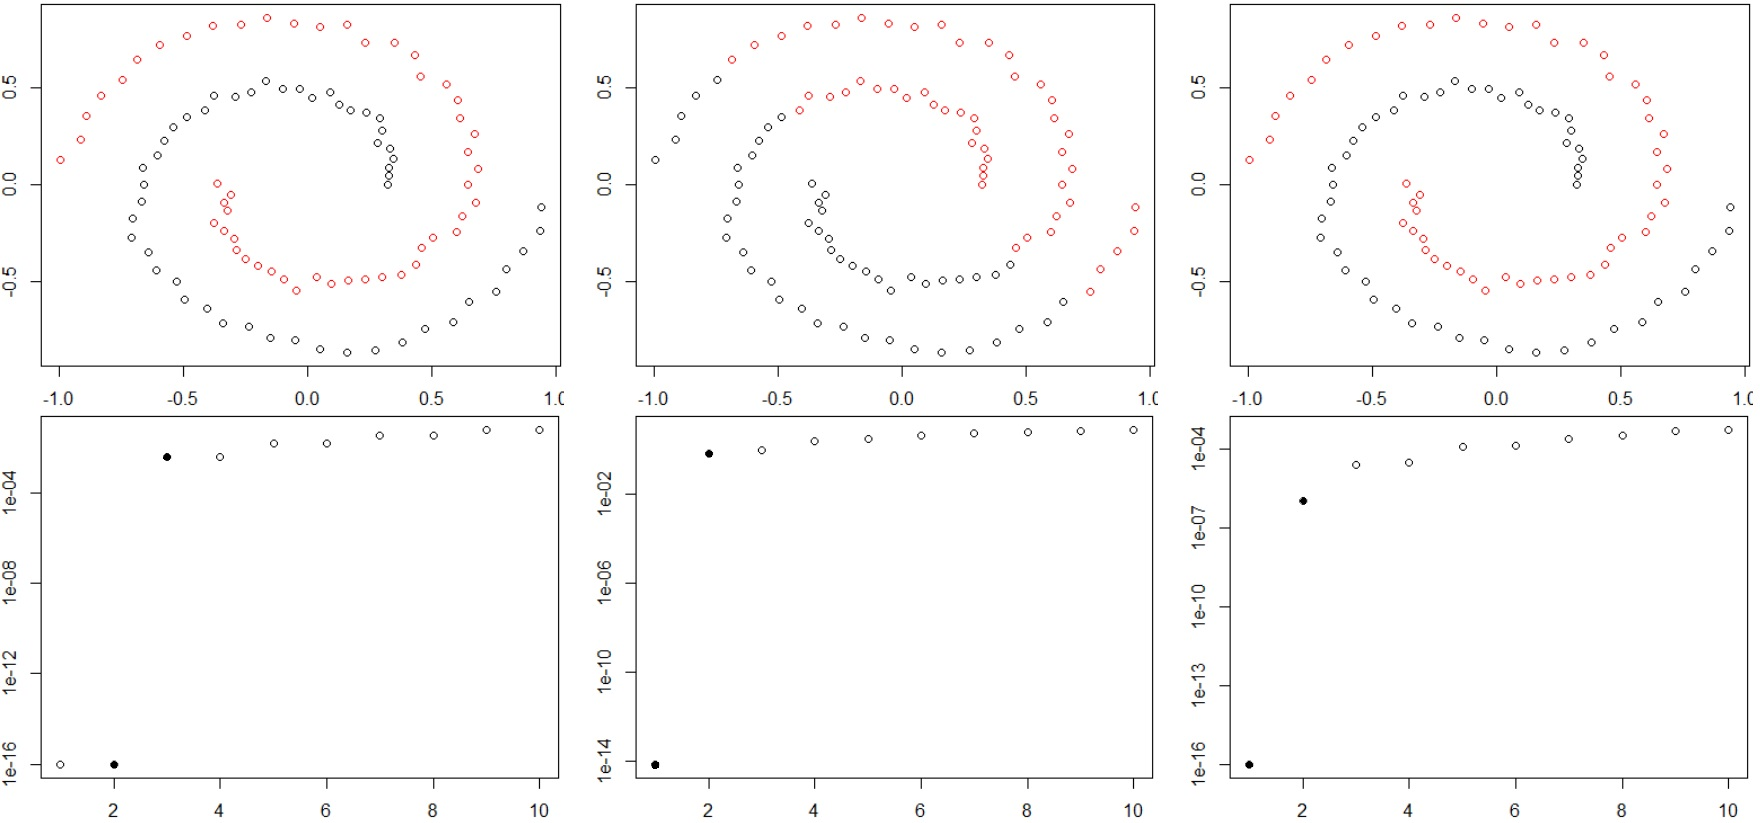
\includegraphics[width=\textwidth]{unnorm-spiral}
\end{figure}

\begin{figure}[h]
\caption{Normaliziran algoritem RW: graf 3-najbližjih sosedov, graf $\epsilon$-ske okolice ($\epsilon$ = 0.4), poln graf ($\delta^2$=0.01)}
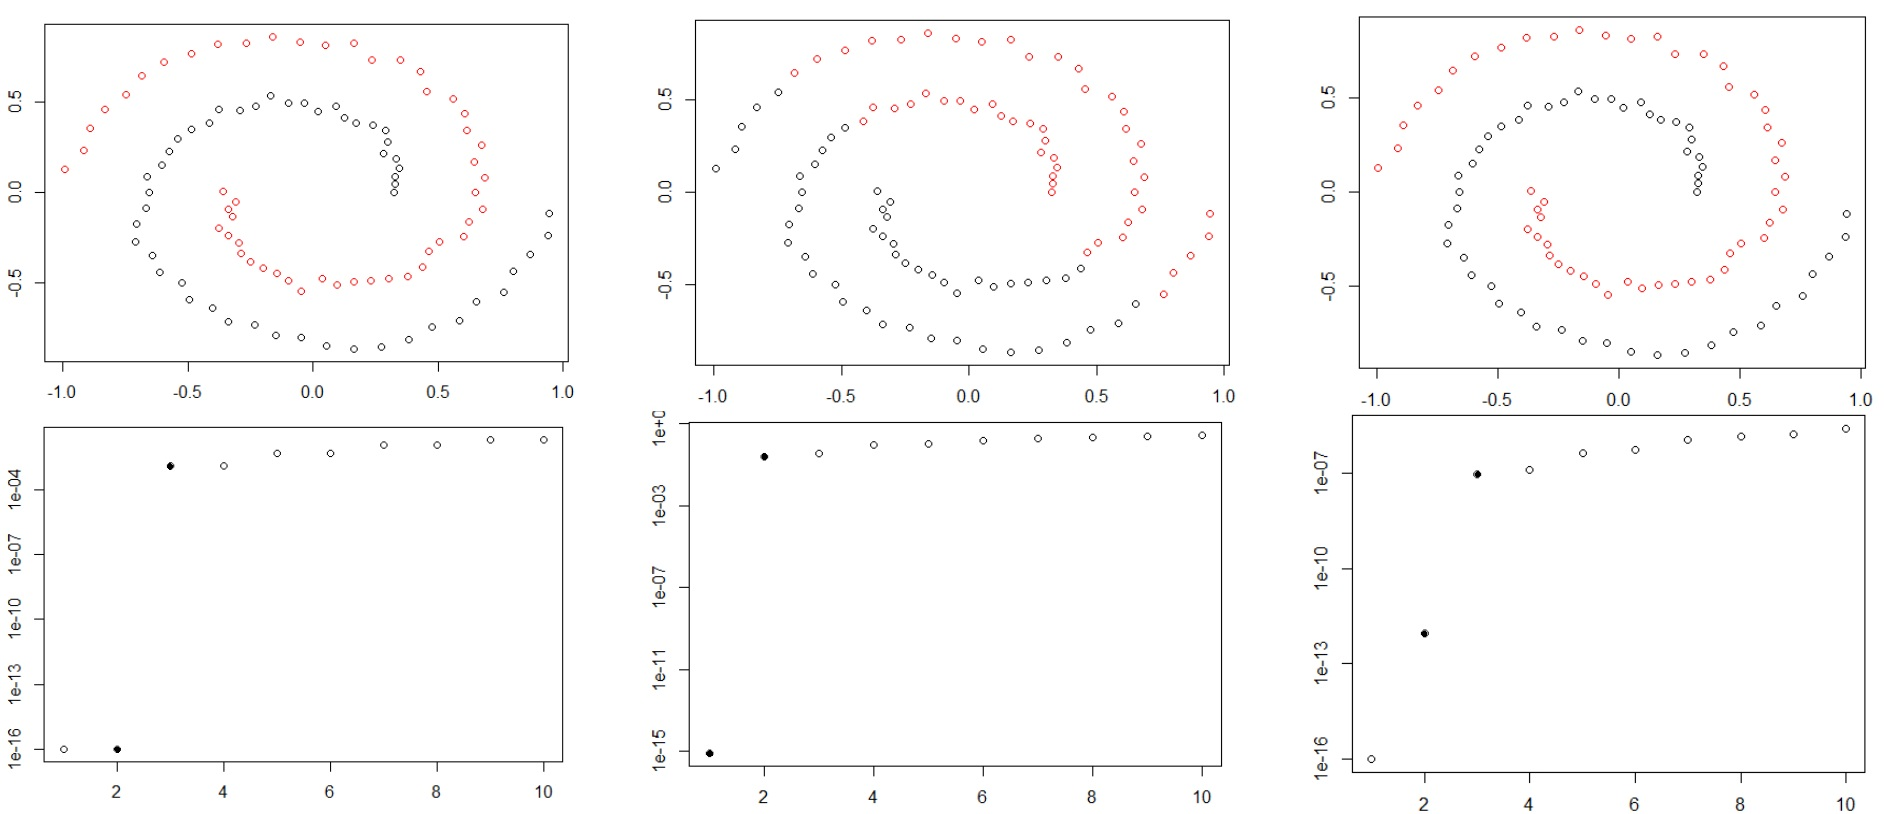
\includegraphics[width=\textwidth]{norm-spiral}
\end{figure}

\begin{figure}[h]
\caption{Normaliziran algoritem SYM: graf 3-najbližjih sosedov, graf $\epsilon$-ske okolice ($\epsilon$ = 0.4), poln graf ($\delta^2$=0.01)}
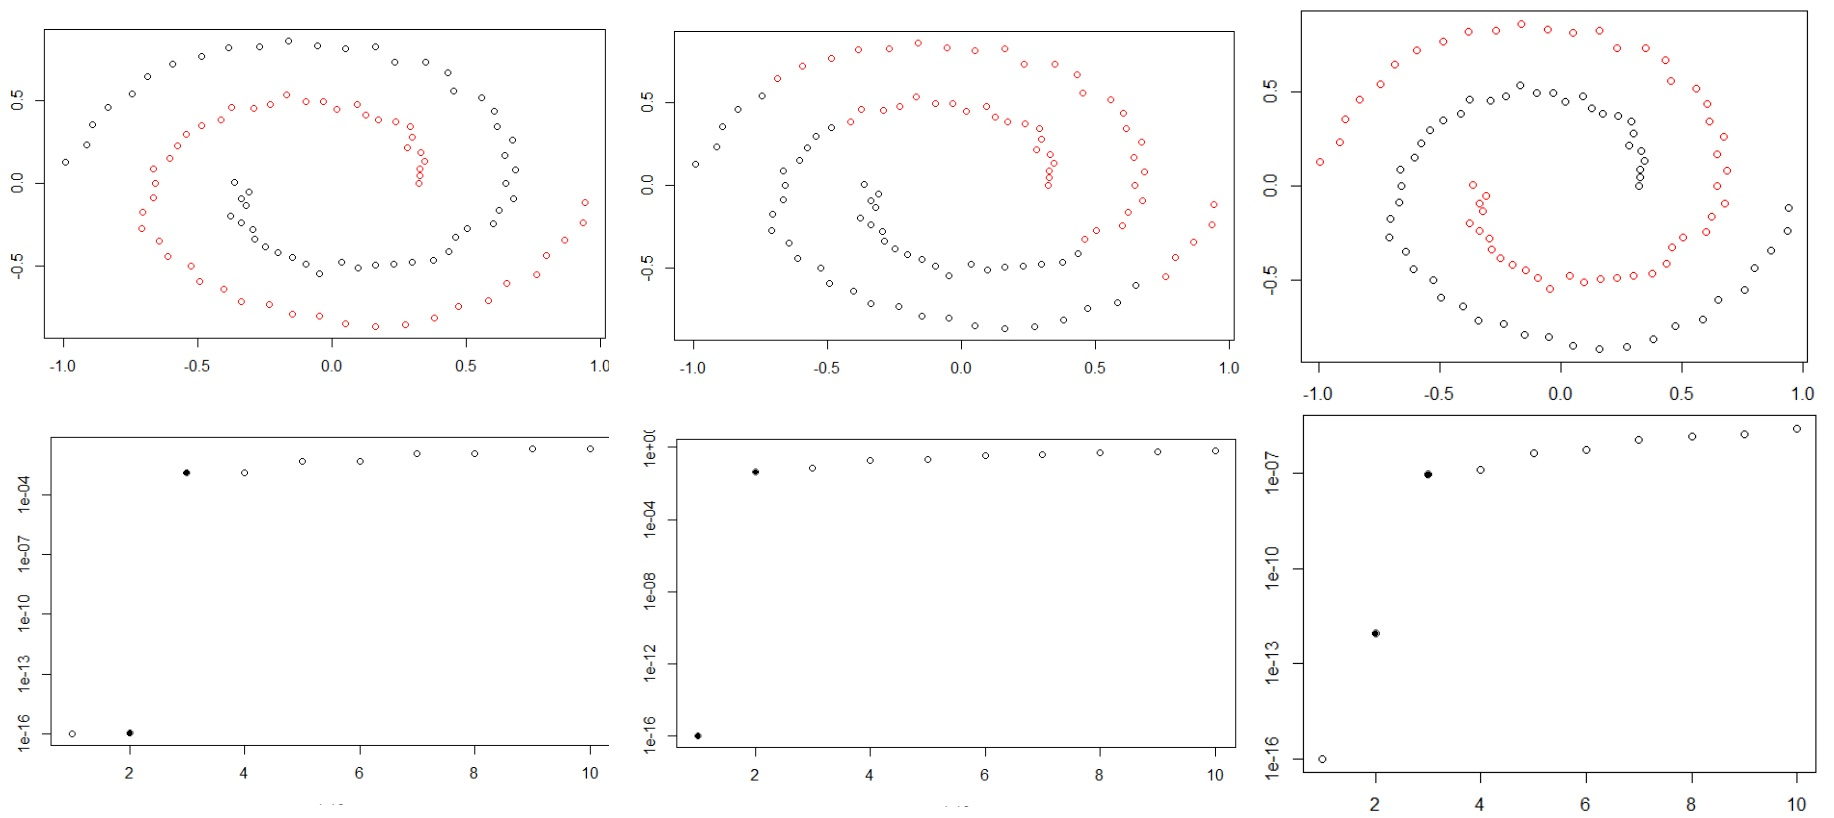
\includegraphics[width=\textwidth]{norm-spiral-sym}
\end{figure}

\begin{figure}[h]
\caption{Nenormaliziran algoritem: graf 3-najbližjih sosedov, graf $\epsilon$-ske okolice ($\epsilon$ = 0.5), poln graf ($\delta^2$=0.01)}
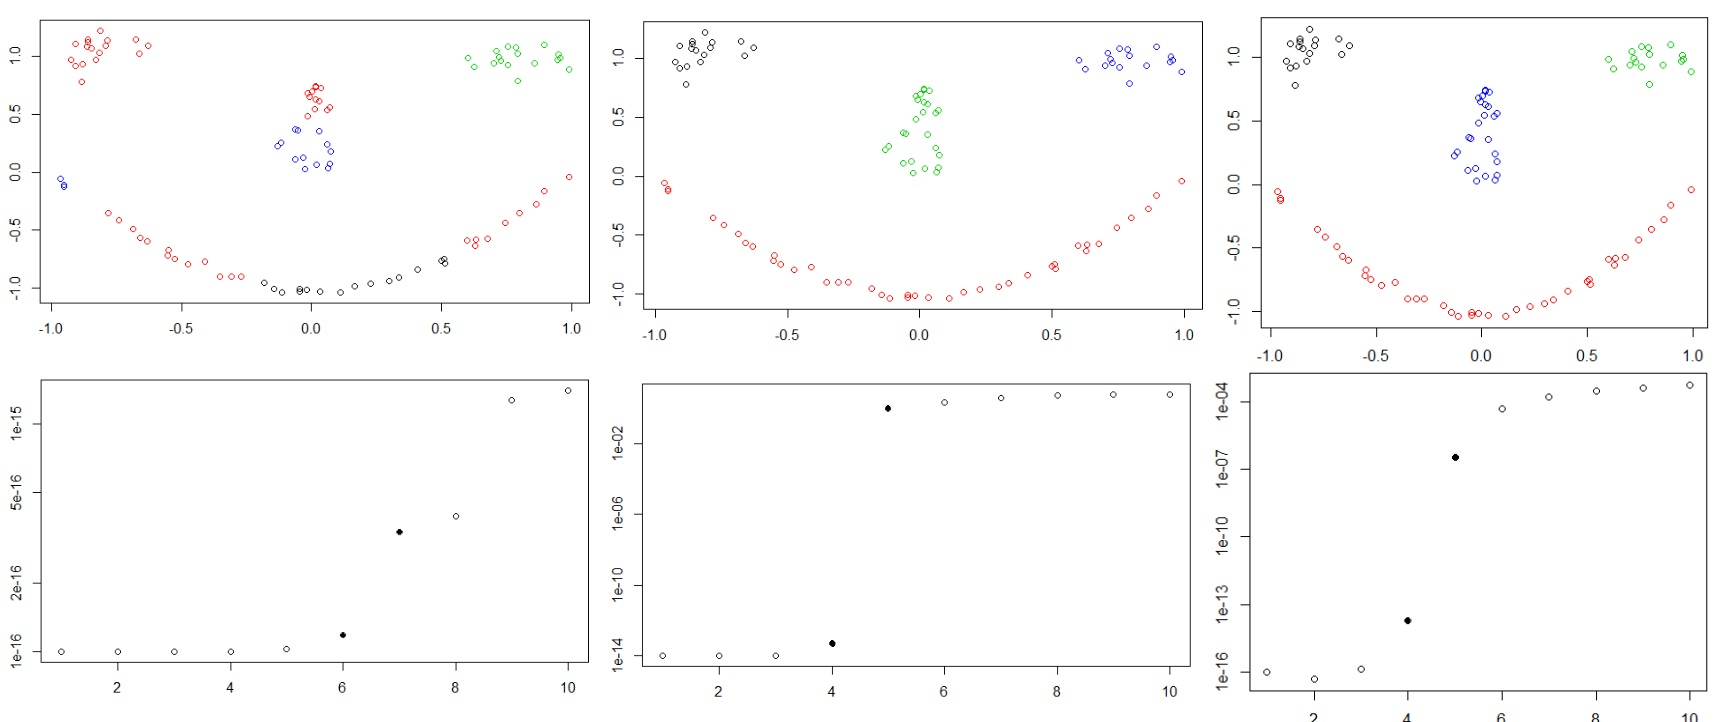
\includegraphics[width=\textwidth]{unnorm-smiley}
\end{figure}

\begin{figure}[h]
\caption{Normaliziran algoritem RW: graf 3-najbližjih sosedov, graf $\epsilon$-ske okolice ($\epsilon$ = 0.5), poln graf ($\delta^2$=0.01)}
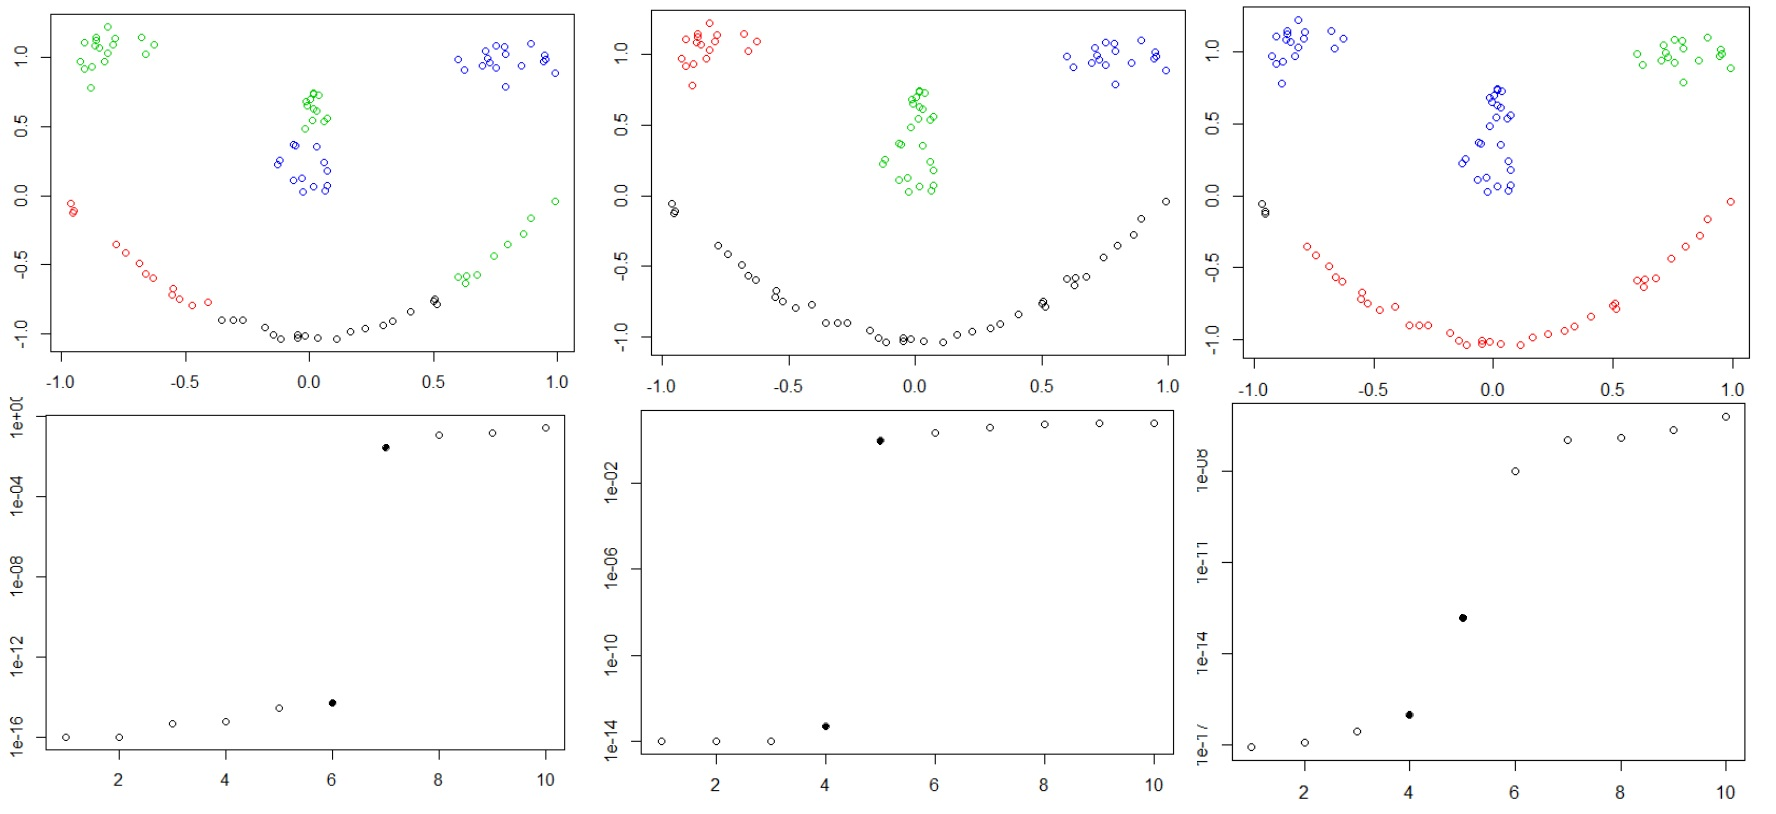
\includegraphics[width=\textwidth]{norm-smiley}
\end{figure}

\begin{figure}[h]
\caption{Normaliziran algoritem SYM: graf 3-najbližjih sosedov, graf $\epsilon$-ske okolice ($\epsilon$ = 0.5), poln graf ($\delta^2$=0.01)}
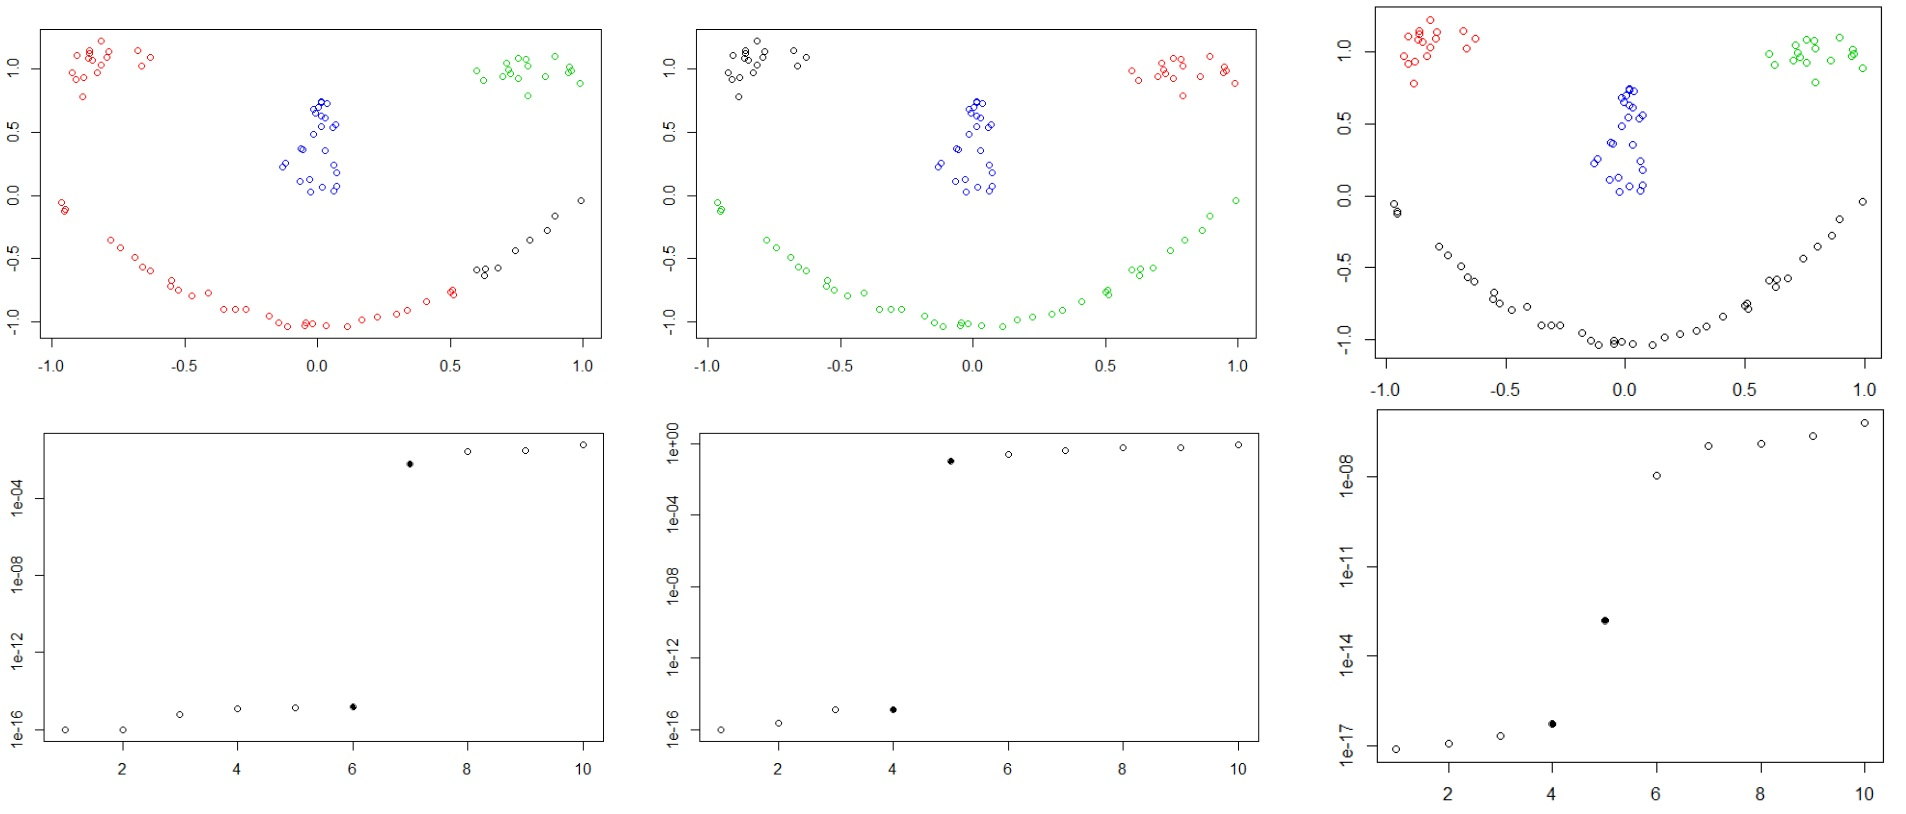
\includegraphics[width=\textwidth]{norm-smiley-sym}
\end{figure}

\begin{figure} [h]
\subsection{Dodaten primer}
Za konec pa smo algoritem poskusili na malo bolj zahtevnem primeru. Zanimalo nas je, kako spektralno grupiranje deluje na slikah - prepoznavanje objektov. Izbrali smo črno-belo sliko in jo pretvorili v matriko, na kateri smo izvedli nenormalizirano spektralno grupiranje z $\delta^2$ = 0.01 (v povezavi z varianco podatkov). Da smo prišli do željenega rezultata, smo morali malo eksperimentirati s parametri. Z rezultatom smo zadovoljni, saj je algoritem zelo dobro ločil objekt od ostalega.\\
\\
\caption{Nenormaliziran algoritem na črno-beli sliki, $k$=3, $\delta^2$ = 0.01}
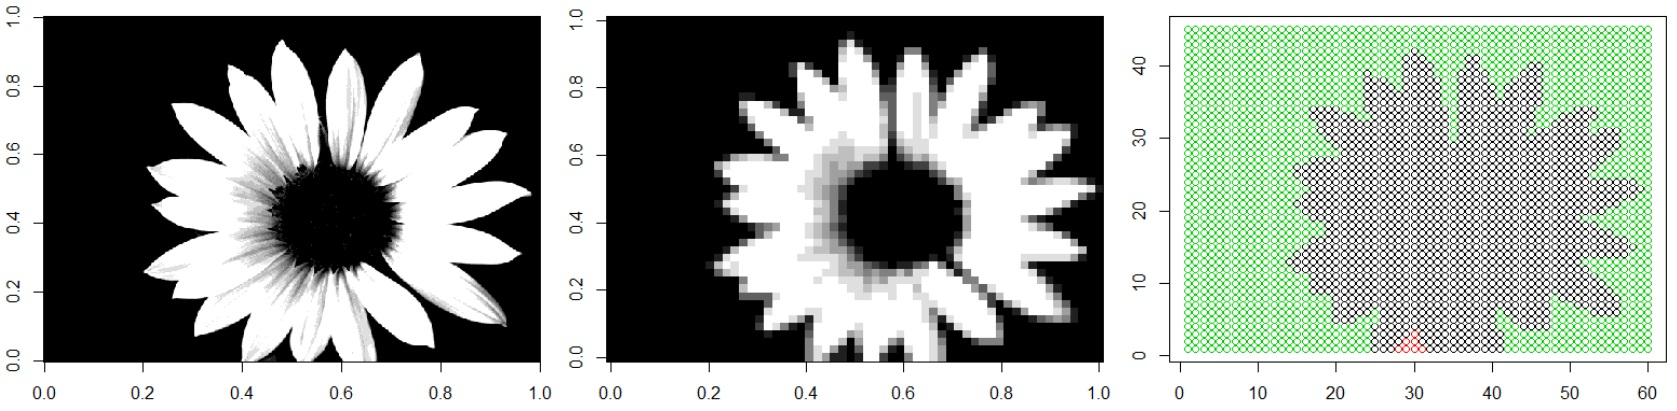
\includegraphics[width=\textwidth]{roza}
\end{figure}




\end{document}

